\documentclass[a4paper]{article}

\usepackage[a4paper, top=8mm, bottom=8mm, left=8mm, right=8mm]{geometry}
\usepackage{float}
\usepackage{graphicx}
\usepackage{booktabs}
\usepackage{multirow}
\usepackage{hyperref}
\usepackage{bookmark}
\usepackage{csquotes}
\usepackage{amsmath}

\usepackage{polyglossia}
\setdefaultlanguage[babelshorthands=true]{russian}
\setotherlanguage{english}

\usepackage{fontspec}
\setmainfont{CMU Serif}
\setsansfont{CMU Sans Serif}
\setmonofont{CMU Typewriter Text}

\usepackage[tiny, compact]{titlesec}
\usepackage{titling}
\setlength{\droptitle}{-1cm}
\pretitle{\begin{center}\begin{bfseries}\Large}
\posttitle{\par\end{bfseries}\end{center}}
\preauthor{\begin{center}\normalsize}
\postauthor{\par\end{center}\vspace{-1.8cm}}

\title{Разреженные матрицы на F\#}

\author{Брулевич Никита Петрович}
\date{}

\begin{document}

\sloppy

\maketitle

\begin{flushright}
    Группа: \emph{2025.Б-73-мм} \\
    Кафедра: \emph{кафедра системного программирования} \\
    Научный руководитель: \emph{Григорьев Семён Вячеславович} \\
    Номер семестра практики: \emph{2}
\end{flushright}

\section*{Введение}

Работа выполнена в рамках проекта LamaGraph (Lambdas, Matrices and Graphs), нацеленного на разработку прототипа вычислителя для разреженной линейной алгебры на основе деревьев квадрантов, реализованного на языке F\#. В рамках проекта разрабатывается библиотека QTreeFSharp, предоставляющая структуры данных для разреженных матриц, векторов и операции над ними.

В соответствии с техническим заданием требовалось реализовать следующие операции: взятие среза для вектора и матрицы (\texttt{Vector.slice}, \texttt{Matrix.slice}), редукция матрицы по строкам и столбцам (\texttt{reduceRows}, \texttt{reduceCols}), произведение Кронекера двух матриц (\texttt{kroneckerProduct}) и поэлементное отображение для матрицы (\texttt{Matrix.map}).

Реализованные операции являются базовыми компонентами библиотеки QTreeFSharp для последующей реализации алгоритмов над разреженными матрицами и графовых алгоритмов в проекте LamaGraph. Полученные результаты необходимы для расширения функциональности библиотеки для её дальнейшего использования в прикладных задачах.

В данном отчёте представлены результаты реализации этих операций, их теоретические свойства и результаты экспериментального исследования выбранных операций на синтетических и реальных разреженных матрицах и векторах.

\section{Постановка задачи}

\textbf{Целью работы} является реализация набора операций над разреженными матрицами и векторами для библиотеки QTreeFSharp в рамках проекта LamaGraph.

Для достижения цели были поставлены следующие задачи:

\begin{enumerate}
    \item реализовать операцию взятия среза для вектора (\texttt{Vector.slice});
    \item реализовать операцию взятия среза для матрицы (\texttt{Matrix.slice});
    \item реализовать редукцию матрицы по строкам (\texttt{reduceRows});
    \item реализовать редукцию матрицы по столбцам (\texttt{reduceCols});
    \item реализовать произведение Кронекера двух матриц (\texttt{kroneckerProduct});
    \item реализовать поэлементное отображение для матрицы (\texttt{Matrix.map});
    \item разработать модульные тесты для всех реализованных операций;
    \item экспериментально проверить теоретические оценки сложности реализованных функций;
    \item экспериментально проверить, какой подход к редукции матрицы по столбцам эффективнее: прямой или через транспонирование с применением редукции по строкам.
\end{enumerate}


\section{Описание предлагаемого решения}

В этом разделе описываются структуры данных, лежащие в основе библиотеки QTreeFSharp, а также детали реализации операций, которые были разработаны в рамках работы.

\subsection{Архитектура QTreeFSharp}

Библиотека QTreeFSharp предоставляет два основных типа данных.

\textbf{Разреженный вектор} представлен бинарным деревом \texttt{btree}, где листья содержат либо \texttt{Dummy} (пустой блок), либо \texttt{UserValue(v)} (значение, применяемое ко всему блоку). Размер хранилища выбирается как наименьшая ближайшая вверх степень двойки, что обеспечивает сбалансированность при рекурсивном спуске.

\textbf{Разреженная матрица} реализована на дереве квадрантов \texttt{qtree} с четырьмя подузлами: NW, NE, SW, SE. Это позволяет рекурсивно делить матрицу на квадранты, а также схлопывать блоки через функцию \texttt{mkNode}, которая превращает четыре одинаковых листа в один.

\subsection{Реализованные операции}

\textbf{Срез вектора (\texttt{Vector.slice}).} Операция вырезает подвектор по заданным границам. Реализация использует две вспомогательные рекурсивные функции: \texttt{narrowOld} (поиск узла старого дерева, покрывающего запрошенный диапазон) и \texttt{buildNewTree} (построение нового дерева из найденного узла). 

Для среза, границы которого совпадают с границами некоторого поддерева, операция выполняется быстрее всего: \texttt{narrowOld} находит это поддерево за время, пропорциональное глубине дерева, после чего \texttt{buildNewTree} обрабатывает найденную структуру. В общем случае стоимость определяется числом узлов результирующего дерева, затронутых построением; верхняя оценка составляет \(O(B \log N)\), где \(B\)~--- число узлов результирующего дерева, \(N\)~--- размер хранилища исходного дерева. На практике для плотных данных наблюдается близкое к линейному масштабирование.

\textbf{Срез матрицы (\texttt{Matrix.slice}).} Операция вырезает подматрицу по заданным границам строк и столбцов. Реализация аналогична векторному срезу, но с учётом двумерной структуры. При выровненном срезе затраты на поиск поддерева минимальны; в общем случае стоимость определяется числом узлов результирующего дерева и дополнительными затратами на обработку границ, что даёт верхнюю оценку \(O(B \log N)\). 

\textbf{Редукция матрицы по строкам и столбцам (\texttt{reduceRows}, \texttt{reduceCols}).} Операции выполняют свёртку матрицы в вектор по строкам и столбцам соответственно. Реализация включает три этапа: обход дерева через \texttt{foldQuadtree}, накопление значений в массиве аккумуляторов и построение результирующего вектора. 

На первом этапе \texttt{foldQuadtree} рекурсивно обходит узлы дерева, включая внутренние узлы и пустые листья, поэтому стоимость этого этапа пропорциональна числу посещённых узлов \(U\). На втором этапе каждый ненулевой элемент обрабатывается один раз, что даёт вклад \(O(nnz)\). На третьем этапе построение вектора через \texttt{fromCoordinateList} включает сортировку координат результата, что добавляет \(O(k \log k)\), где \(k\) — число ненулевых элементов в результате, не превосходящее длину вектора \(n\). 

Таким образом, верхняя оценка всей операции составляет \(O(U + nnz + n\log n)\). В экспериментах на реальных матрицах доминирующий вклад даёт обработка ненулевых элементов, поэтому наблюдаемое время согласуется с \(O(nnz)\).

Для сравнения был реализован альтернативный подход: \texttt{reduceCols} через транспонирование матрицы и последующий \texttt{reduceRows}. Стоимость транспонирования пропорциональна числу узлов исходного дерева. Это позволило оценить эффективность прямой реализации против комбинированного подхода.

\textbf{Произведение Кронекера (\texttt{kroneckerProduct}).} Для каждой пары ненулевых элементов матриц \(A\) и \(B\) вычисляется один элемент результирующей матрицы. Поэтому основная вычислительная часть имеет сложность \(O(nnz(A)\cdot nnz(B))\). Полученные элементы затем распределяются по квадрантам результирующего дерева; в худшем случае этот этап требует \(O(nnz(A)\cdot nnz(B)\cdot \log(n_A n_B))\) операций. 

\textbf{Поэлементное отображение для матрицы (\texttt{Matrix.map}).} Операция применяет переданную функцию к каждому блоку дерева, сложность определяется числом узлов дерева. Эта операция не включена в экспериментальную часть, так как её производительность не являлась предметом исследования, однако функциональная корректность проверена тестами.

\subsection{Тестирование}

Для каждой реализованной функции были написаны модульные тесты. Общее количество тестов:
\begin{itemize}
    \item \texttt{Vector.slice}~--- 11 тестов;
    \item \texttt{Matrix.slice}~--- 22 теста;
    \item \texttt{Matrix.reduceRows} / \texttt{reduceCols}~--- 14 тестов;
    \item \texttt{Matrix.kroneckerProduct}~--- 13 тестов;
    \item \texttt{Matrix.map}~--- 6 тестов.
\end{itemize}

Все тесты успешно проходят. Для оценки полноты тестирования был выполнен замер покрытия кода с использованием встроенного инструмента .NET (\texttt{dotnet test --collect "XPlat Code Coverage"}). Результаты показывают, что все ключевые реализованные операции имеют высокое покрытие:
\begin{itemize}
    \item \texttt{Vector.slice}~--- 100\% строк и веток;
    \item \texttt{Matrix.slice}~--- 100\% строк и веток;
    \item \texttt{Matrix.kroneckerProduct}~--- 100\% строк и веток;
    \item \texttt{Matrix.reduceRows} / \texttt{reduceCols}~--- 96\% строк (не покрыта только защитная ветка обработки ошибки при создании вектора, которая недостижима при корректном использовании).
\end{itemize}

Тесты покрывают основные сценарии использования, включая краевые случаи (пустые матрицы, вырожденные срезы, нулевые плотности).

\section{Эксперимент}

В данном разделе описываются условия проведения экспериментов, используемые метрики, а также приводятся результаты замеров производительности реализованных операций.

\subsection{Условия эксперимента}

Все замеры производительности выполнялись с использованием библиотеки BenchmarkDotNet v0.15.8 на физической машине с процессором AMD Ryzen 7 260 (8 ядер, 16 потоков) и 32 ГБ оперативной памяти. 

Для экспериментов с редукциями использовались 30 реальных матриц из коллекции SuiteSparse.

Для операций взятия среза использовались синтетические векторы и матрицы разных плотностей и размеров. Параметры синтетических данных:
\begin{itemize}
    \item \texttt{Vector.slice}: размеры \(4\cdot10^6\), \(5\cdot10^6\), \(7.5\cdot10^6\), \(10^7\), \(1.25\cdot10^7\); плотности 0.01, 0.05, 0.1, 0.25, 0.5;
    \item \texttt{Matrix.slice}: размеры 1000, 2000, 3000, 4000, 5000, 6000, 7000; плотности 0.001, 0.005, 0.01, 0.05, 0.1, 0.5.
\end{itemize}

Для \texttt{kroneckerProduct}: размеры A и B принимают значения 150, 200, 250, 300; плотность A фиксирована на 0.01, плотность B варьируется 0.005, 0.01, 0.05, 0.1. 

Для оценки устойчивости результатов использовались 10 фиксированных начальных значений генератора псевдослучайных чисел (seed) (0--9). Для синтетических benchmark'ов на графиках приведены средние значения Mean по десяти seed.

Для измерения эффекта выравнивания слайсов был проведён отдельный диагностический эксперимент при фиксированном seed = 0 на матрице 4096×4096 с плотностями 0.001--0.5 и смещениями начала среза 0, 1, 512, 1024, 1536, 2048. Для вектора аналогичный эксперимент проведён на векторе \(4\cdot10^6\) элементов с теми же плотностями и смещениями 0, 1, 512.

\subsection{Метрики}

В качестве метрик использовались среднее время выполнения (Mean) в миллисекундах и объём выделенной памяти (Allocated) в мегабайтах, измеренные BenchmarkDotNet. Показатель Allocated характеризует суммарный объём управляемой памяти, выделенной во время выполнения benchmark, и не является пиковым потреблением памяти. В таблицах приведены средние значения (Mean) и стандартные отклонения (StdDev), рассчитанные по результатам измерительных итераций.

\subsection{Статистическая проверка теоретических оценок}

Для проверки теоретических оценок, приведённых в разделе~2, использовалась линейная регрессия в лог-лог координатах. Идея метода состоит в следующем: если время работы подчиняется степенной зависимости
\[
T = c \cdot X^k,
\]
то после логарифмирования получается линейное соотношение
\[
\log T = \log c + k \log X,
\]
где наклон \(k\) соответствует показателю степени в исходной зависимости.

Поскольку все оценки в разделе~2 являются верхними, в качестве \(X\) выбиралась функция от размера входа, пропорциональная теоретической оценке:
\begin{itemize}
    \item для \texttt{Matrix.slice} (\(O(B \log N)\)), где \(B \sim \text{Size}^2\) при фиксированной плотности, в качестве предиктора использовалась \(\text{Size}^2 \cdot \log_2(\text{Size})\);
    \item для \texttt{Vector.slice} (\(O(B \log N)\)), где \(B \sim \text{Size}\), в качестве предиктора использовалась \(\text{Size} \cdot \log_2(\text{Size})\);
    \item для \texttt{kroneckerProduct} (\(O(nnz(A) \cdot nnz(B))\)) в качестве предиктора использовалась \(nnz(A) \cdot nnz(B)\);
    \item для \texttt{reduceRows} / \texttt{reduceCols} в качестве основного предиктора использовалась \(nnz\) (доминирующая компонента оценки \(O(U + nnz + n \log n)\)). Дополнительно проверялся предиктор \(nnz \cdot \log_2 n\), учитывающий рекурсивную фильтрацию координат в \texttt{fromCoordinateList}.
\end{itemize}

Если теоретическая оценка верна, наклон \(k\) должен быть близок к 1. Для оценки адекватности модели вычислялись коэффициент детерминации \(R^2\), 95\% доверительный интервал для \(k\) и \(p\)-value для гипотезы о том, что истинный наклон равен 1.

Для редукций использовались точные значения \(nnz\), \(nrows\), \(ncols\), извлечённые из файлов, содержащих реальные матрицы коллекции SuiteSparse.

\subsection{Результаты}

\textbf{Сравнение прямой редукции и подхода с транспонированием}

Цель этого эксперимента~--- сравнить эффективность прямой реализации \texttt{reduceCols} и подхода с предварительным транспонированием.

Таблица~\ref{tab:reduce_comparison} показывает сравнение времени выполнения \texttt{reduceCols} (прямая редукция по столбцам) и альтернативного подхода: транспонирование + \texttt{reduceRows}.

\begin{table}[H]
\centering
\caption{Сравнение прямой редукции по столбцам и подхода с транспонированием (Mean $\pm$ StdDev)}
\label{tab:reduce_comparison}
\begin{tabular}{lrrrr}
\toprule
Матрица & Плотность & \texttt{reduceCols} (мс) & Транспонирование + \texttt{reduceRows} (мс) & Соотношение \\
\midrule
bcsstk01 & 19.70\% & 0.024 $\pm$ 0.001 & 0.036 $\pm$ 0.002 & 1.5$\times$ \\
bcsstk13 & 2.85\% & 6.504 $\pm$ 0.080 & 14.564 $\pm$ 0.118 & 2.2$\times$ \\
bcsstk16 & 2.47\% & 22.522 $\pm$ 0.120 & 46.253 $\pm$ 0.453 & 2.1$\times$ \\
bcsstk29 & 0.31\% & 43.003 $\pm$ 0.449 & 60.264 $\pm$ 0.600 & 1.4$\times$ \\
email-Eu-core & 2.53\% & 2.744 $\pm$ 0.025 & 8.183 $\pm$ 0.188 & 3.0$\times$ \\
\bottomrule
\end{tabular}
\end{table}

Во всех 30 случаях прямая редукция по столбцам оказалась быстрее, чем подход с транспонированием. Отношение времени составило от 1.25$\times$ до 2.98$\times$. Медианное отношение~--- 1.74$\times$. Дополнительная стоимость транспонирования приводит к тому, что комбинированный вариант оказывается медленнее прямой реализации.

Из рис.~\ref{fig:reduce_all_time_bar} и рис.~\ref{fig:reduce_all_memory_bar} видно, что прямая реализация быстрее альтернативной на всех исследованных матрицах, при этом она также требует меньших аллокаций.

Для проверки теоретической оценки сложности редукций была построена регрессия времени от числа ненулевых элементов. Полученный наклон составил \(k = 1.10\), 95\% доверительный интервал \([1.01, 1.19]\), \(R^2 = 0.958\). Значение \(k\), близкое к единице, согласуется с доминирующей линейной зависимостью от \(nnz\). Высокое значение \(R^2\) подтверждает адекватность модели.

\begin{figure}[H]
    \centering
    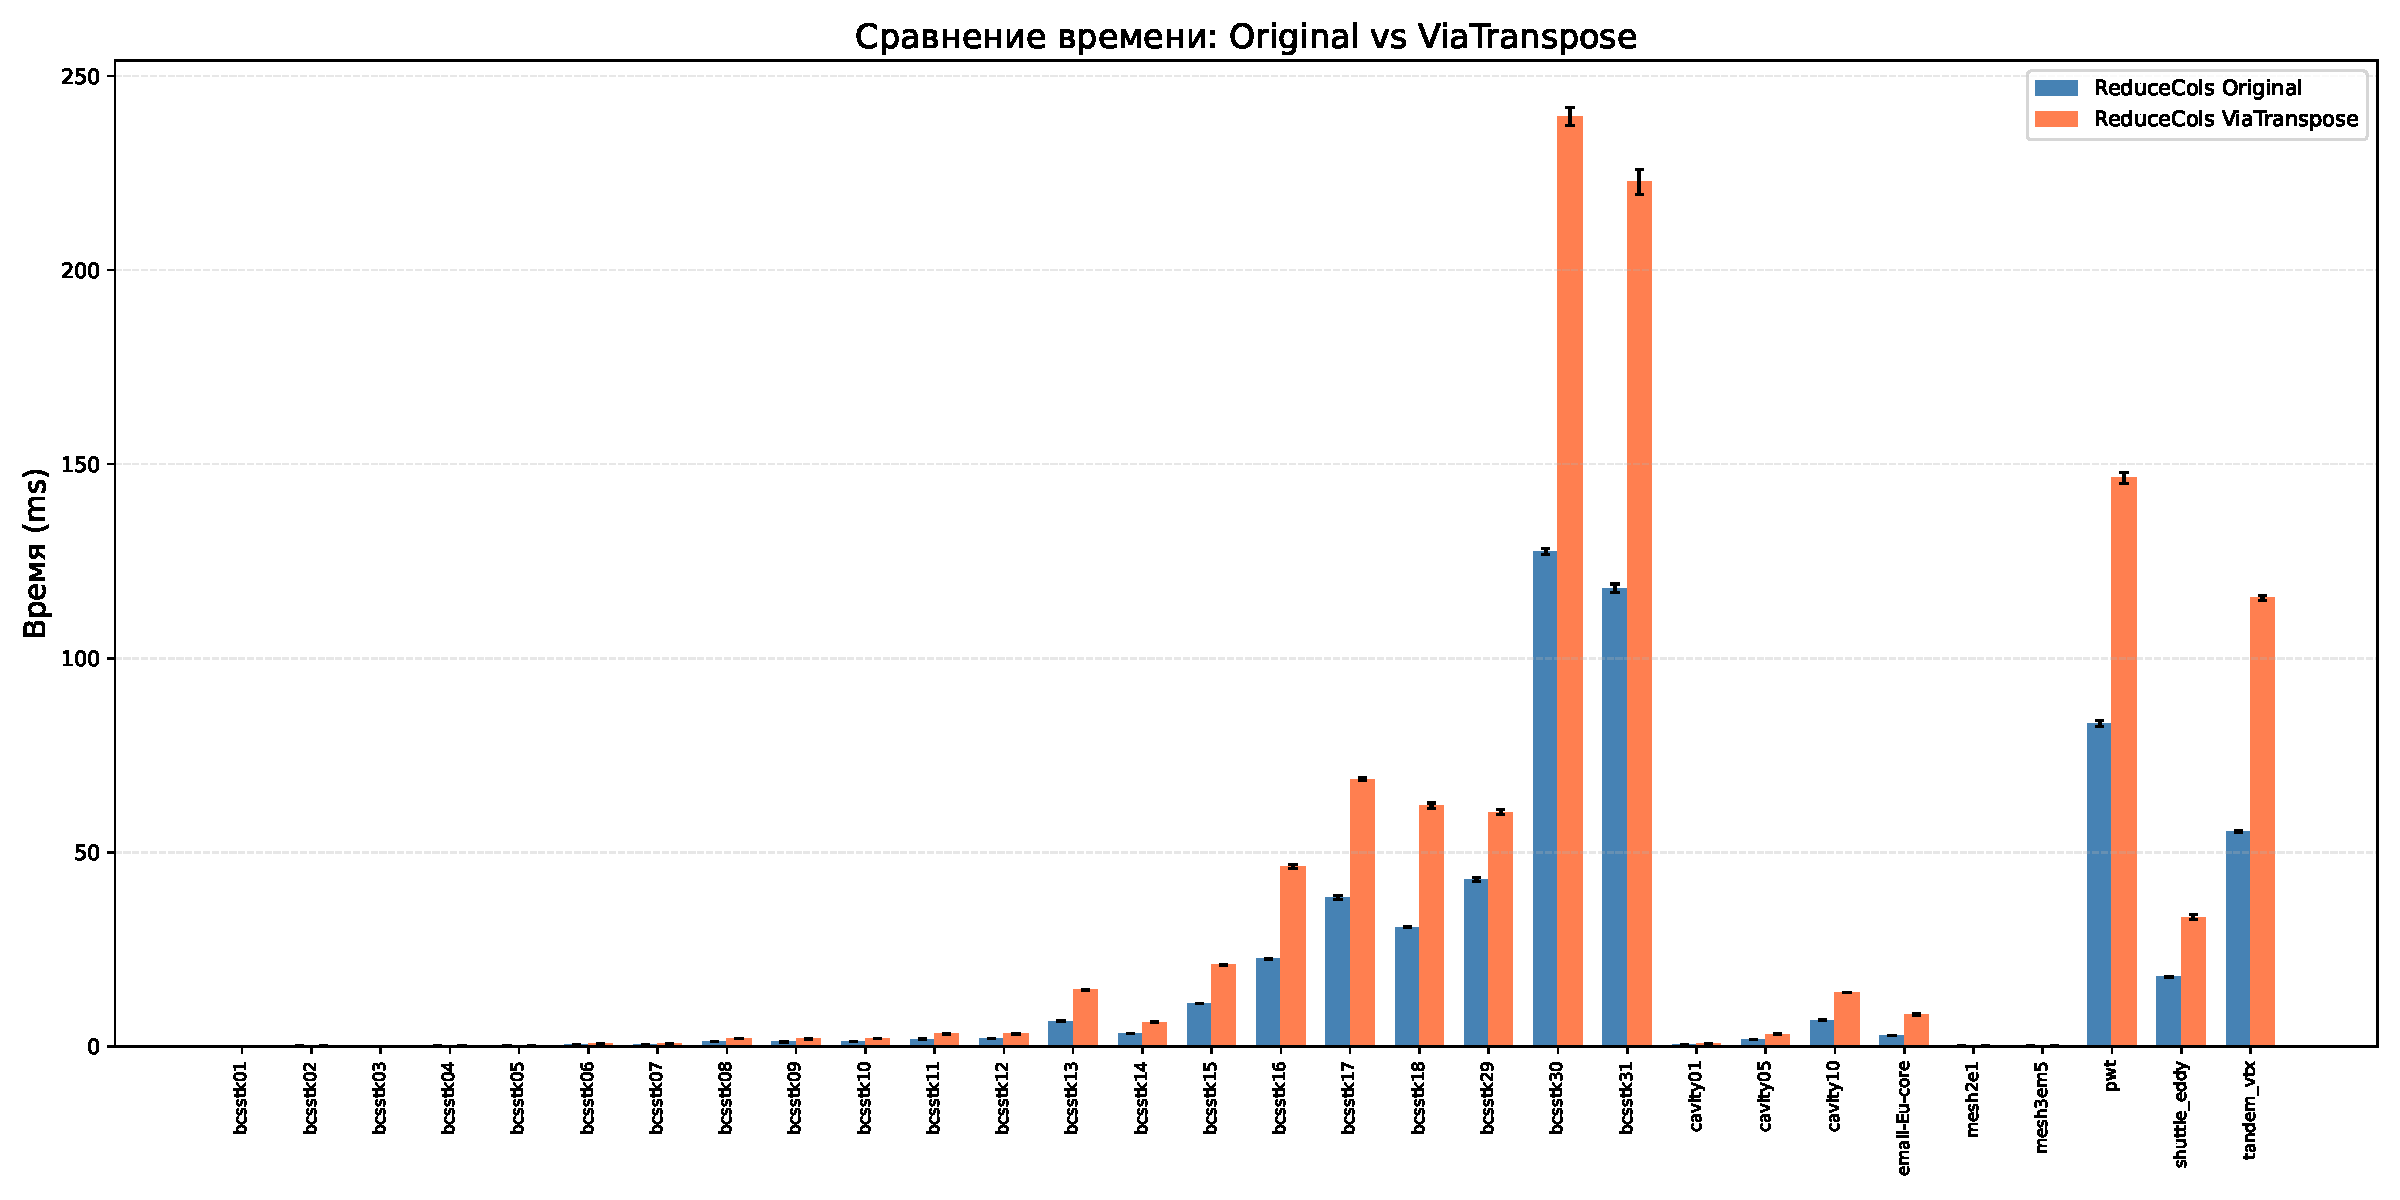
\includegraphics[width=0.9\textwidth]{reduce_all_time_bar.pdf}
    \caption{Сравнение времени выполнения прямой редукции по столбцам и подхода с транспонированием на 30 реальных матрицах}
    \label{fig:reduce_all_time_bar}
\end{figure}

\begin{figure}[H]
    \centering
    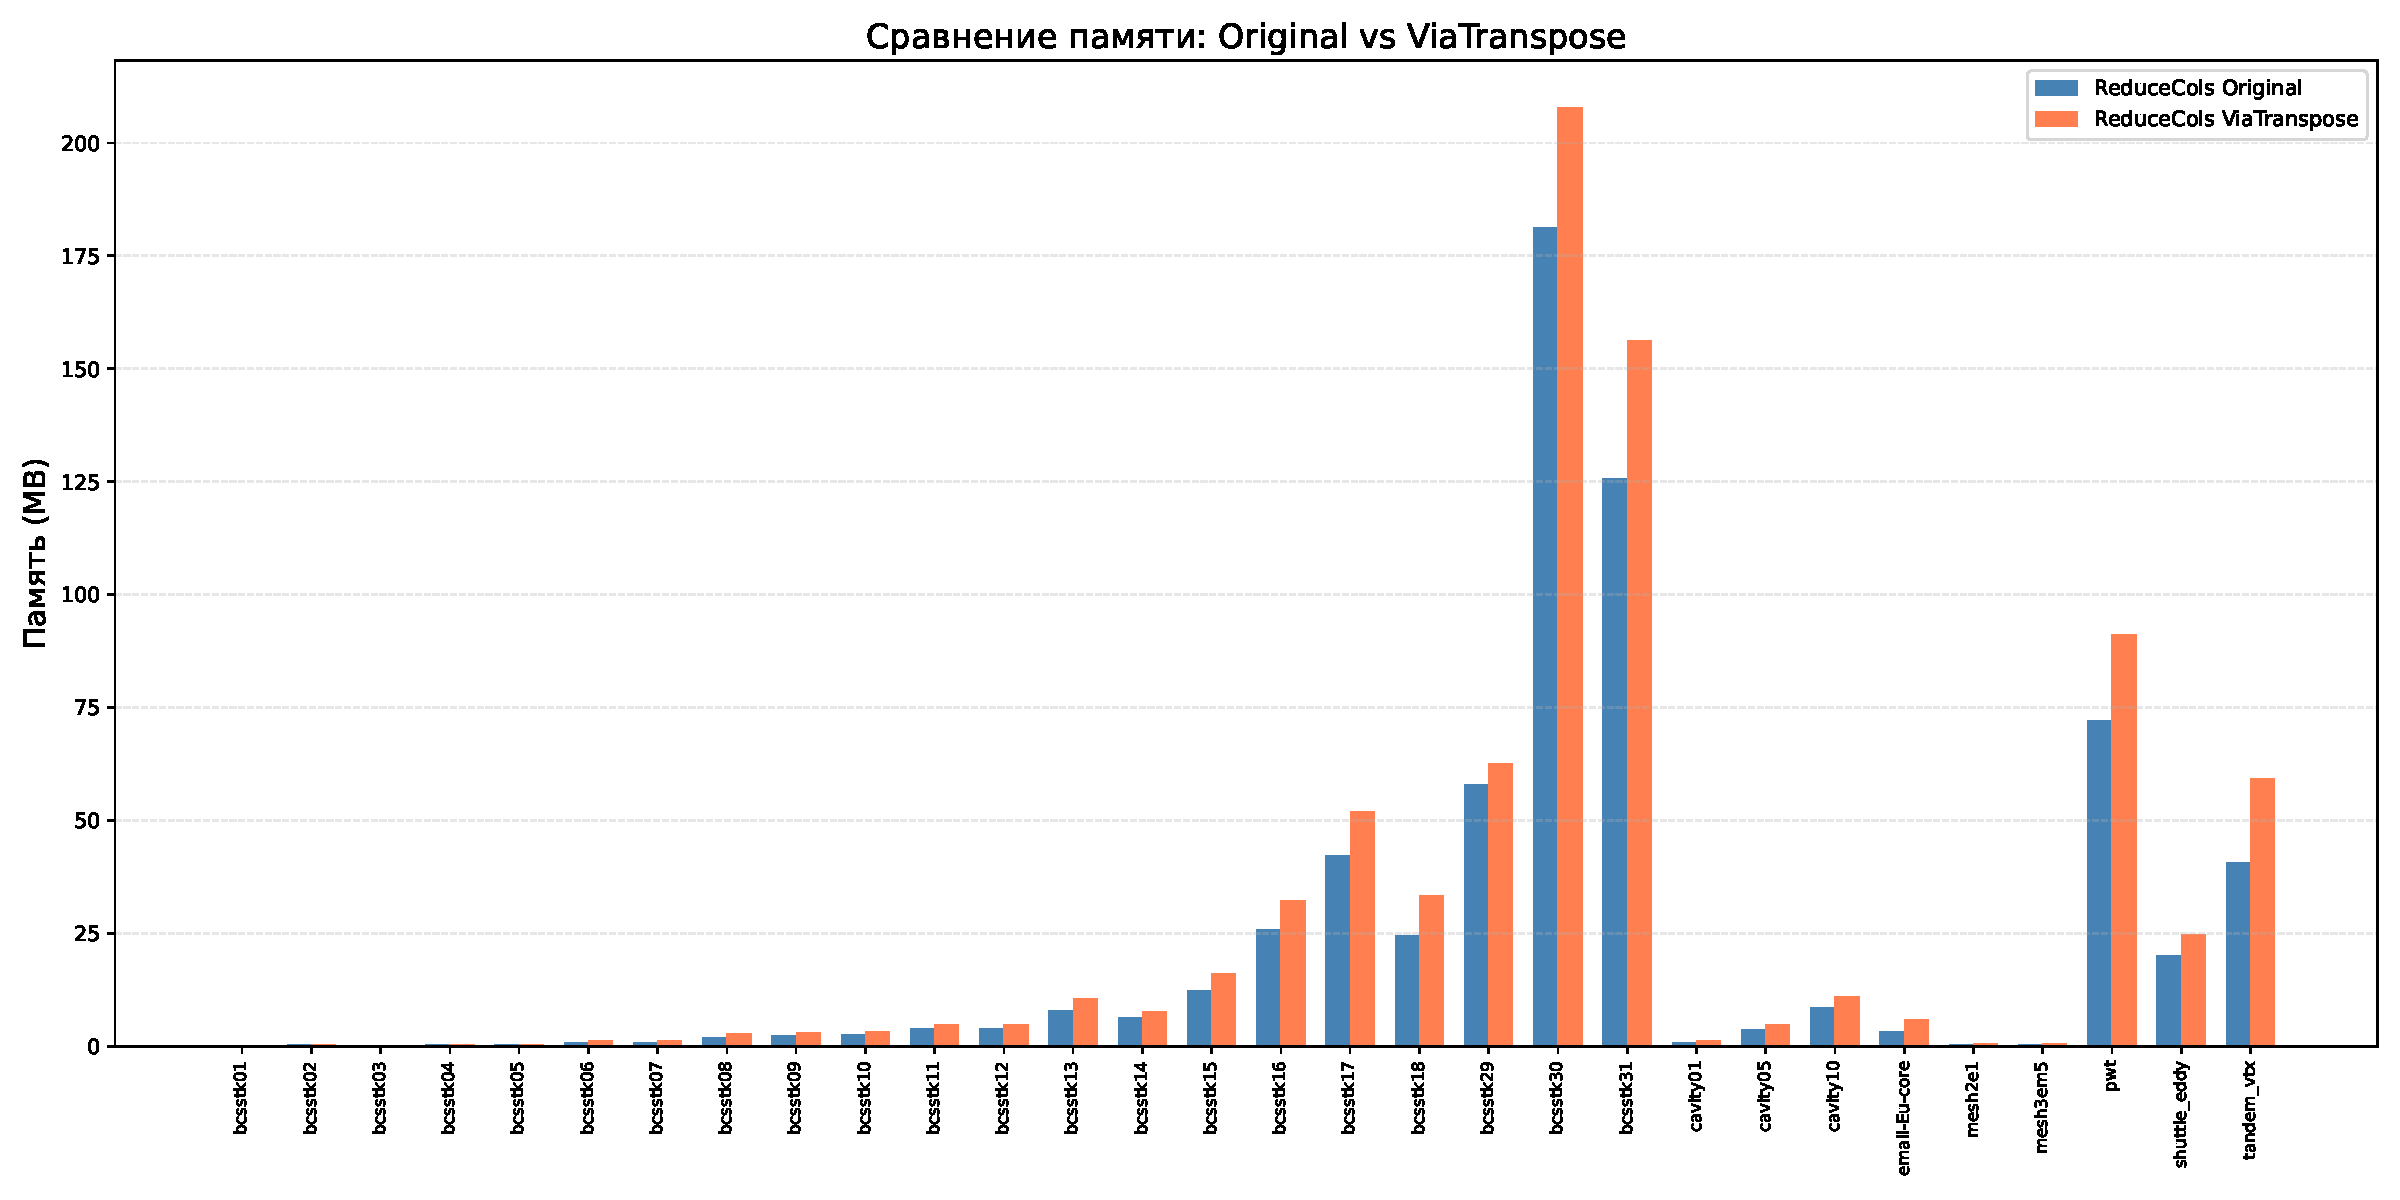
\includegraphics[width=0.9\textwidth]{reduce_all_memory_bar.pdf}
    \caption{Сравнение объёма выделенной памяти для прямой редукции по столбцам и подхода с транспонированием}
    \label{fig:reduce_all_memory_bar}
\end{figure}

\textbf{Масштабирование операций произведения Кронекера и взятия среза}

\textbf{Kronecker.} Цель этого эксперимента~--- исследовать, как время выполнения \texttt{kroneckerProduct} зависит от размеров входных матриц и плотности матрицы (B). Плотность матрицы (A) фиксирована на уровне (0.01), размеры обеих матриц варьируются. Для каждой фиксированной пары (SizeA) и (DensityB) изменение размера (B) позволяет оценить влияние его размера на время выполнения операции.

Для проверки теоретической оценки \(O(nnz(A) \cdot nnz(B))\) была построена регрессия времени от произведения числа ненулевых элементов обеих матриц. Полученный наклон составил \(k = 0.89\), 95\% доверительный интервал \([0.88, 0.90]\), \(R^2 = 0.977\). Поскольку оценка является верхней, значение \(k < 1\) не противоречит теории: реальное время растёт медленнее верхней оценки. Это может объясняться схлопыванием блоков в функции \texttt{mkNode}, из-за которого число обрабатываемых пар меньше, чем \(nnz(A) \cdot nnz(B)\).

\begin{figure}[H]
    \centering
    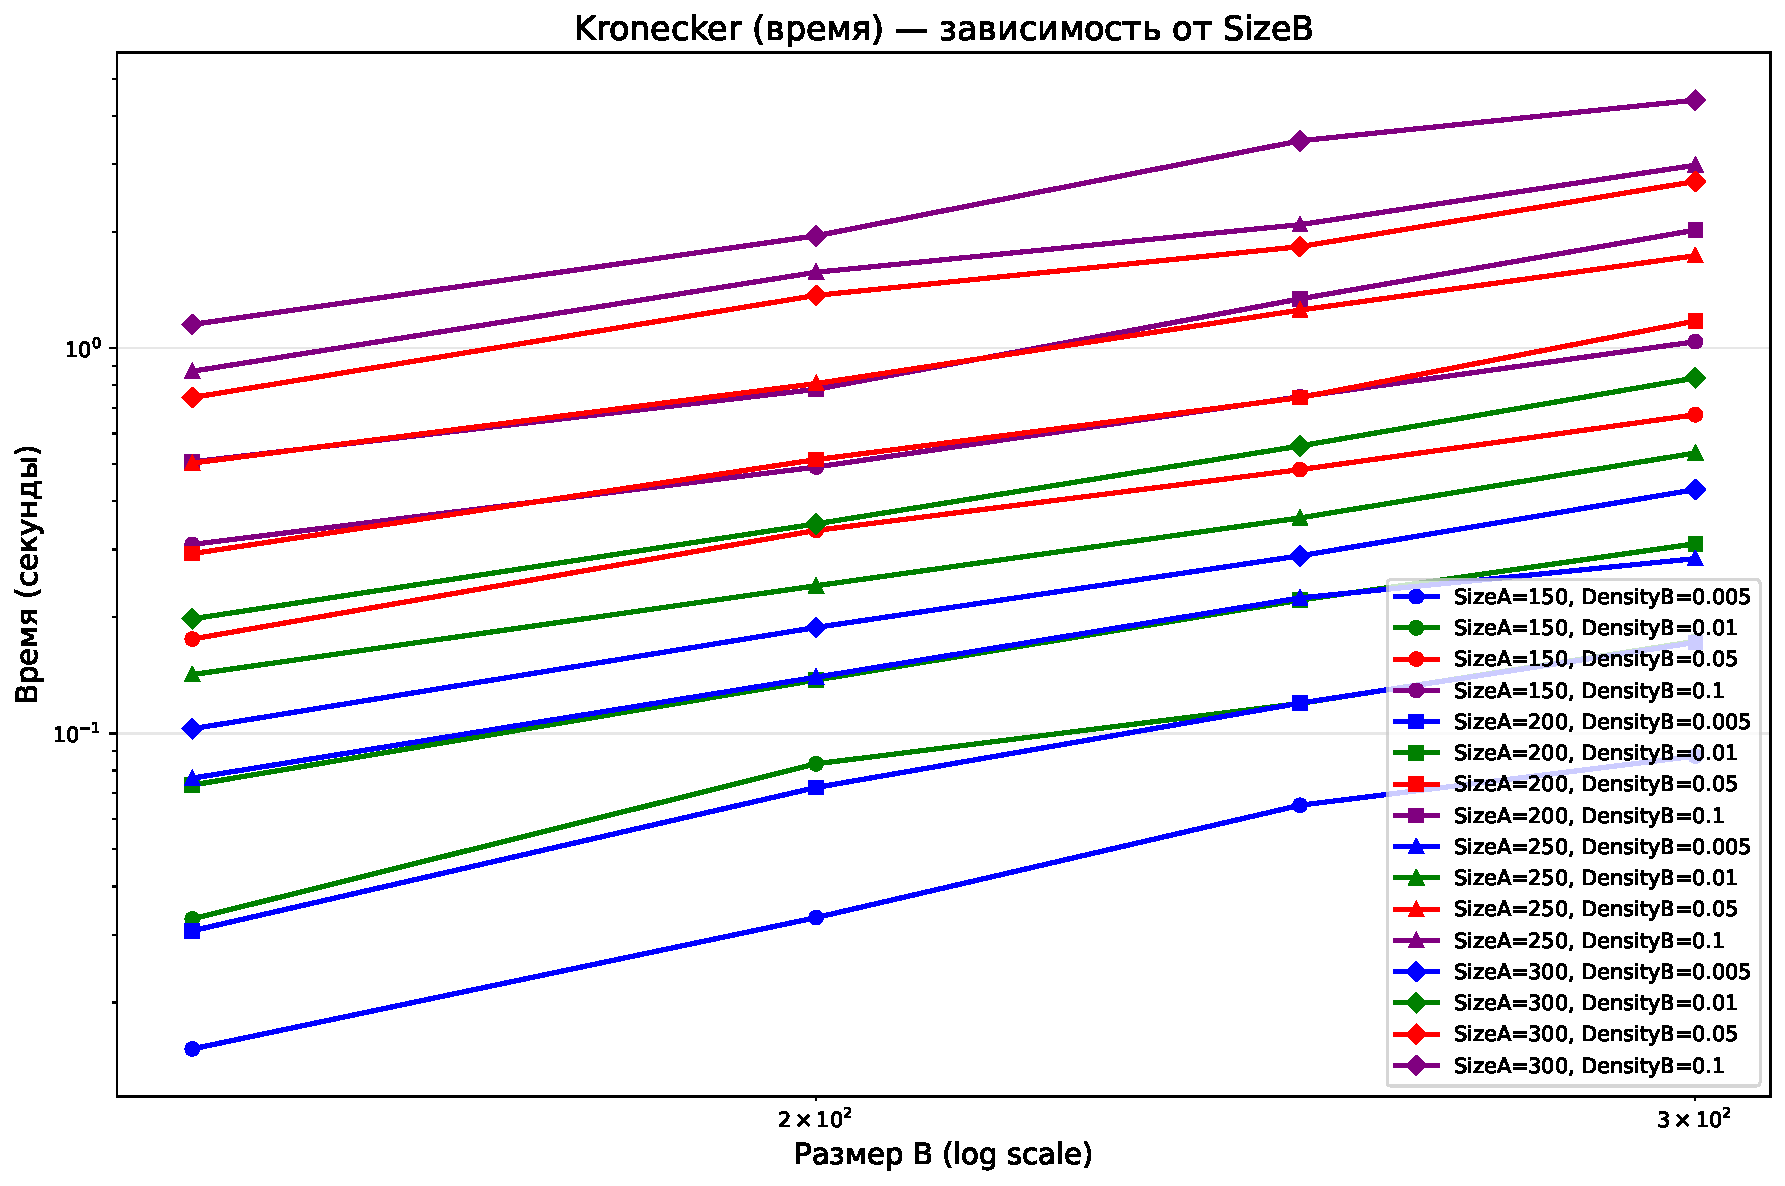
\includegraphics[width=0.9\textwidth]{kronecker_time_vs_sizeB.pdf}
    \caption{Зависимость времени Kronecker от размера B при фиксированном размере A}
    \label{fig:kronecker_time_vs_sizeB}
\end{figure}

\begin{figure}[H]
    \centering
    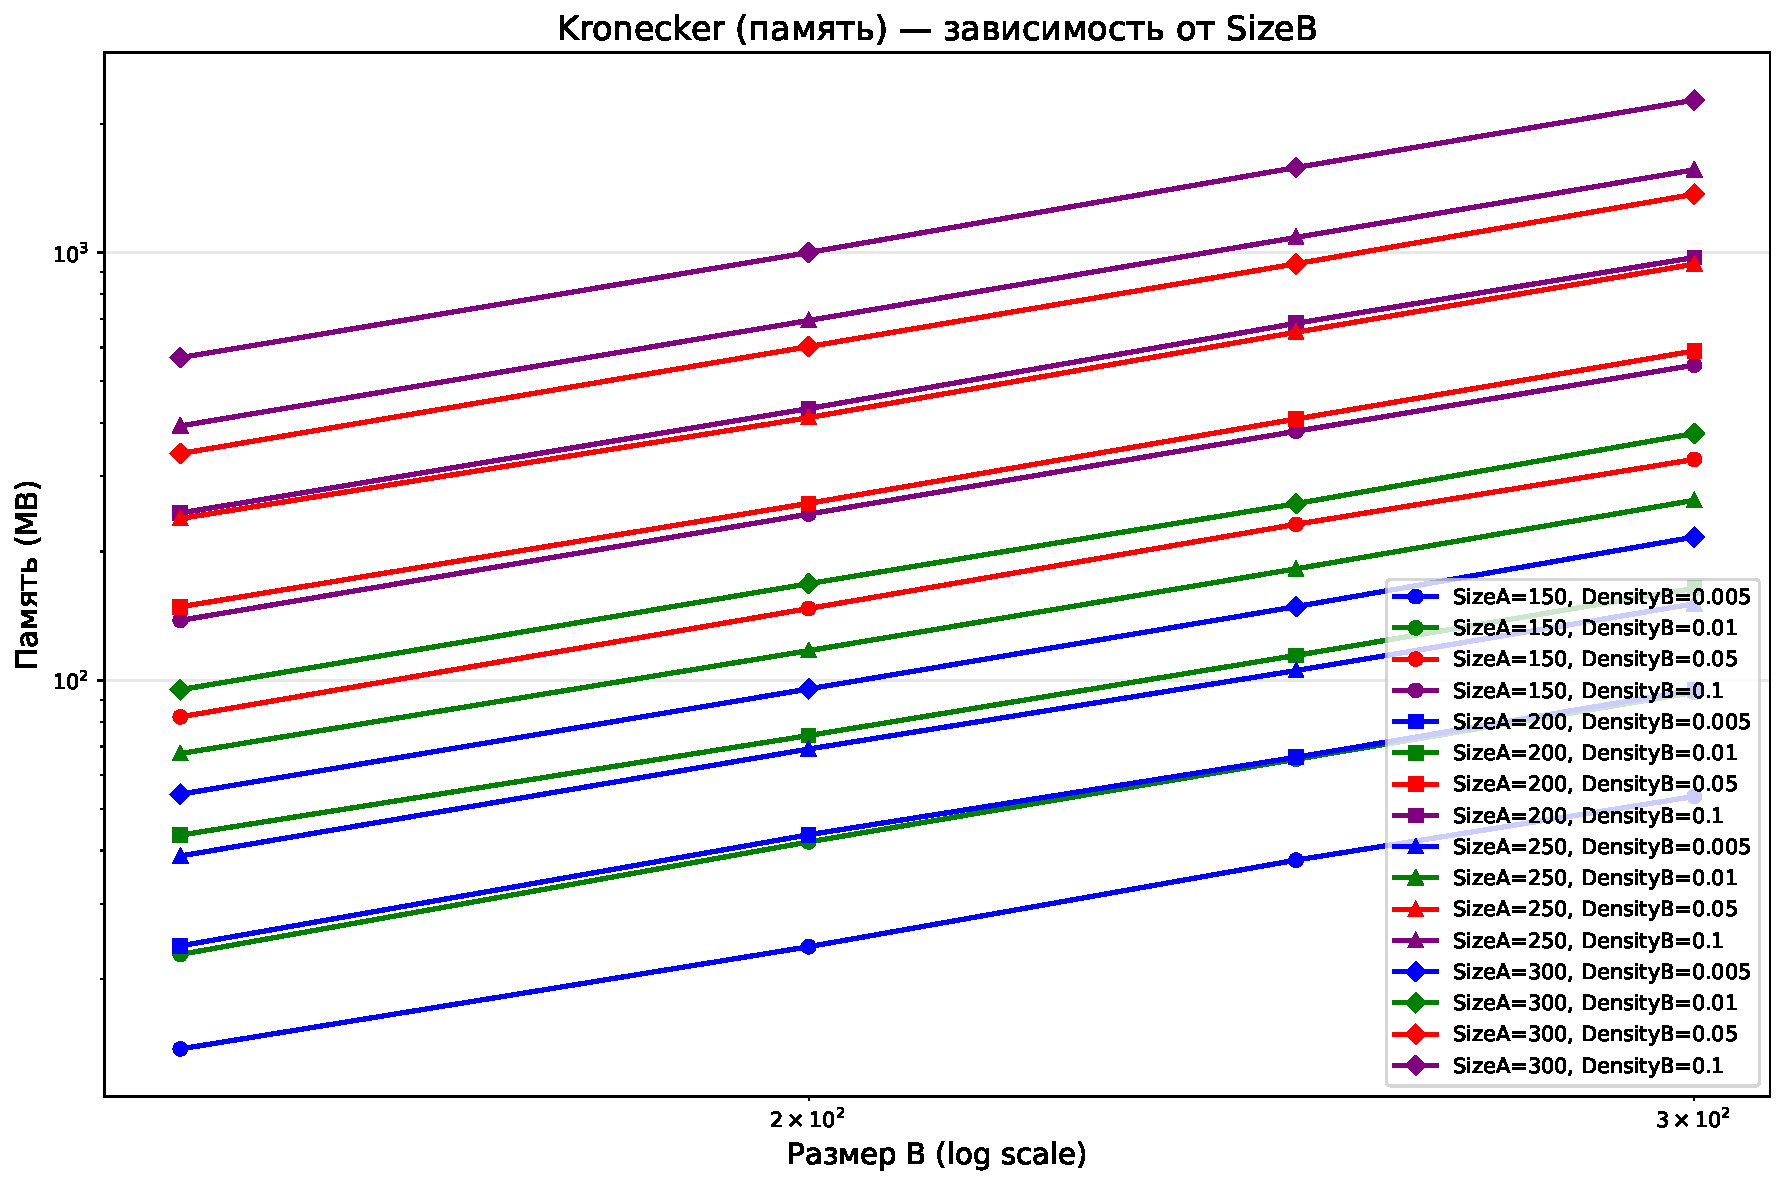
\includegraphics[width=0.9\textwidth]{kronecker_memory_vs_sizeB.pdf}
    \caption{Зависимость аллокаций Kronecker от размера B при фиксированном размере A}
    \label{fig:kronecker_memory_vs_sizeB}
\end{figure}

Из графиков видно, что увеличение размеров входных матриц и плотности (B) приводит к росту времени выполнения и объёма выделенной памяти. Наблюдаемое поведение согласуется с тем, что основная вычислительная часть операции обрабатывает пары ненулевых элементов двух входных матриц, а их число растёт с увеличением размеров и плотности матриц. Это соответствует основной составляющей асимптотической оценки (O(nnz(A)\cdot nnz(B))).

\textbf{Vector.slice.} Цель этого эксперимента~--- проверить масштабирование времени выполнения \texttt{Vector.slice} с размером вектора при различных плотностях. При высоких плотностях (0.25--0.5) наблюдается близкое к линейному масштабирование времени с размером вектора. При снижении плотности степень зависимости возрастает, что  связано с особенностями структуры разреженного бинарного дерева.

Для проверки теоретической оценки \(O(B \log N)\) была построена регрессия времени от предиктора \(\text{Size} \cdot \log_2(\text{Size})\). При плотностях \(\ge 0.1\) полученный наклон \(k\) лежит в диапазоне 0.99--1.03, что согласуется с теоретическим значением \(k = 1\). При плотности 0.01 наблюдается отклонение: \(k = 1.69\), 95\% доверительный интервал \([1.35, 2.02]\). Это объясняется тем, что при низкой плотности число узлов результата \(B\) растёт быстрее, чем \(\text{Size}\), из-за большого количества \texttt{Dummy}-узлов, которые не схлопываются, а также присутствует эффект выравнивания границ среза (см. раздел~\ref{sec:alignment}).

\begin{figure}[H]
    \centering
    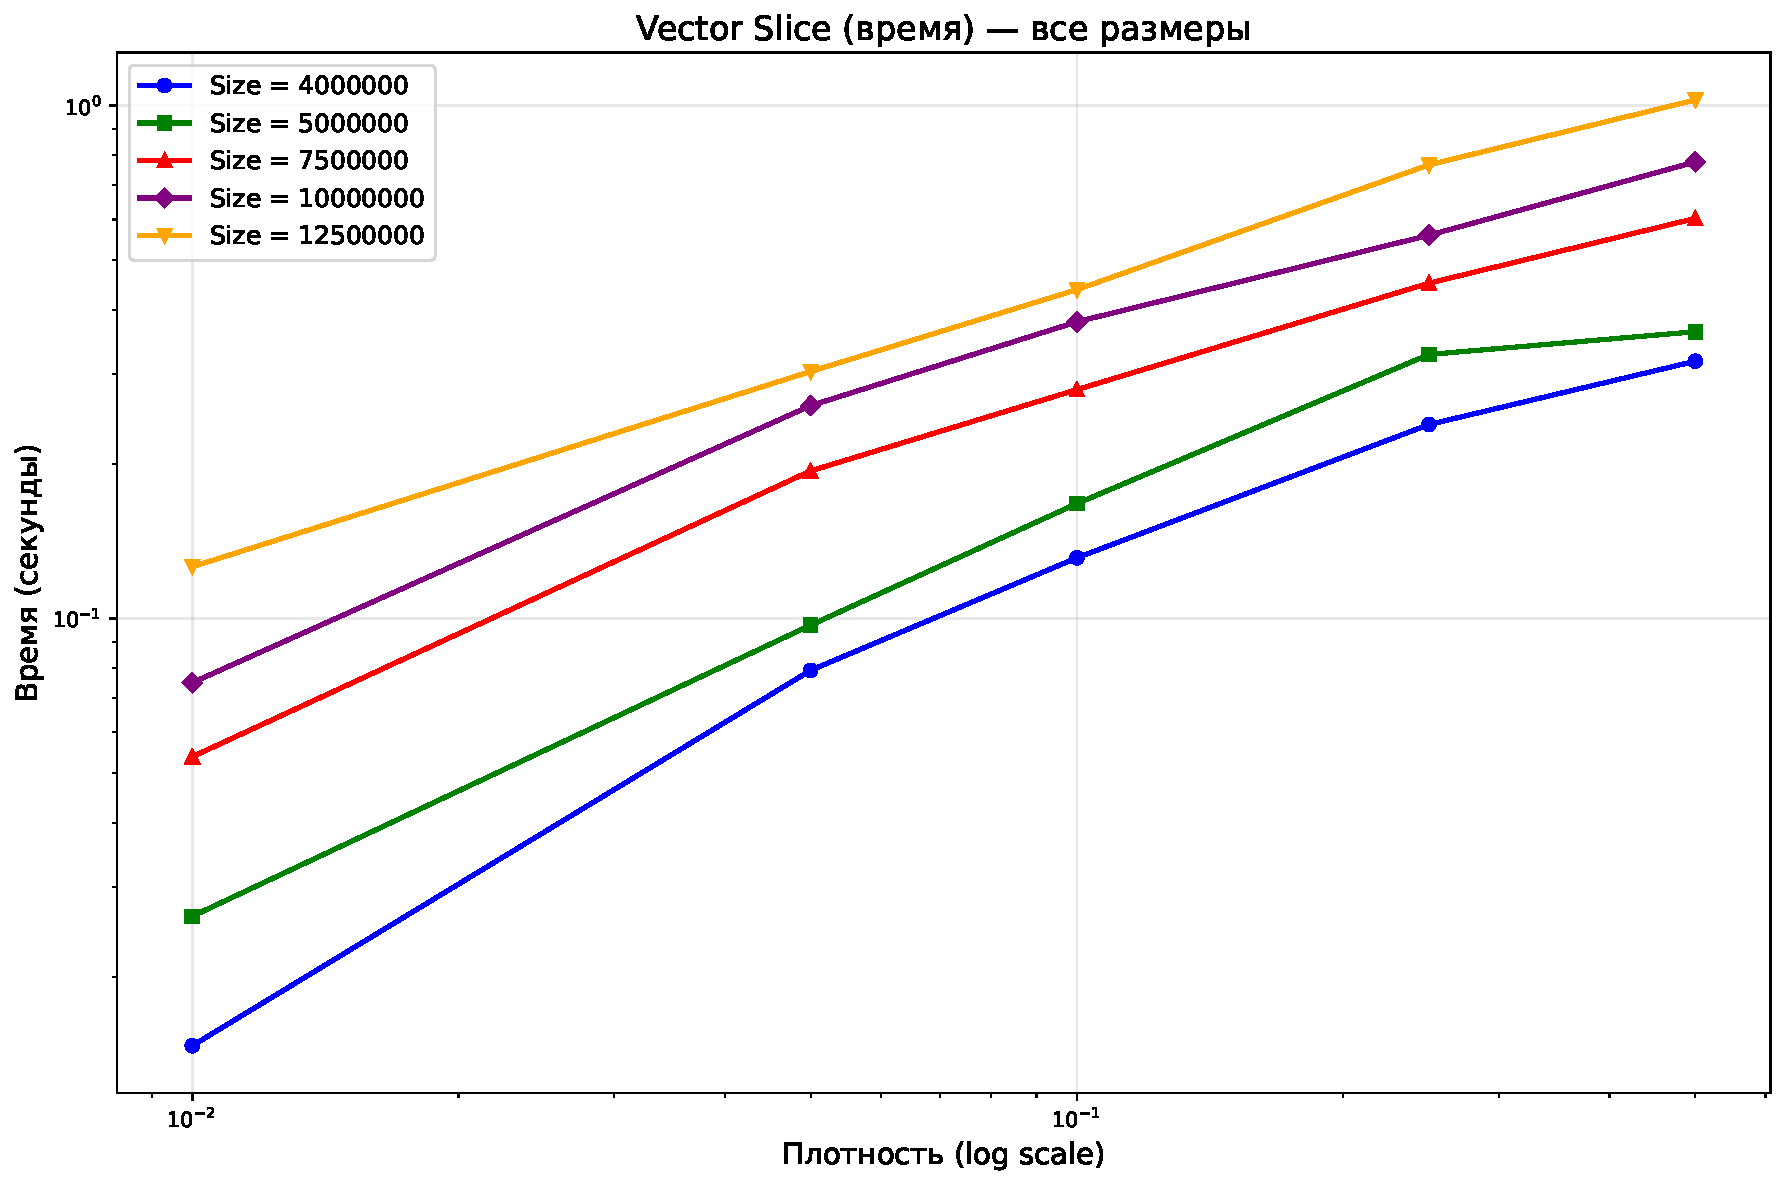
\includegraphics[width=0.9\textwidth]{vector_slice_time_all_sizes.pdf}
    \caption{VectorSlice: время выполнения в зависимости от плотности для различных размеров}
    \label{fig:vector_slice_time_all_sizes}
\end{figure}

\begin{figure}[H]
    \centering
    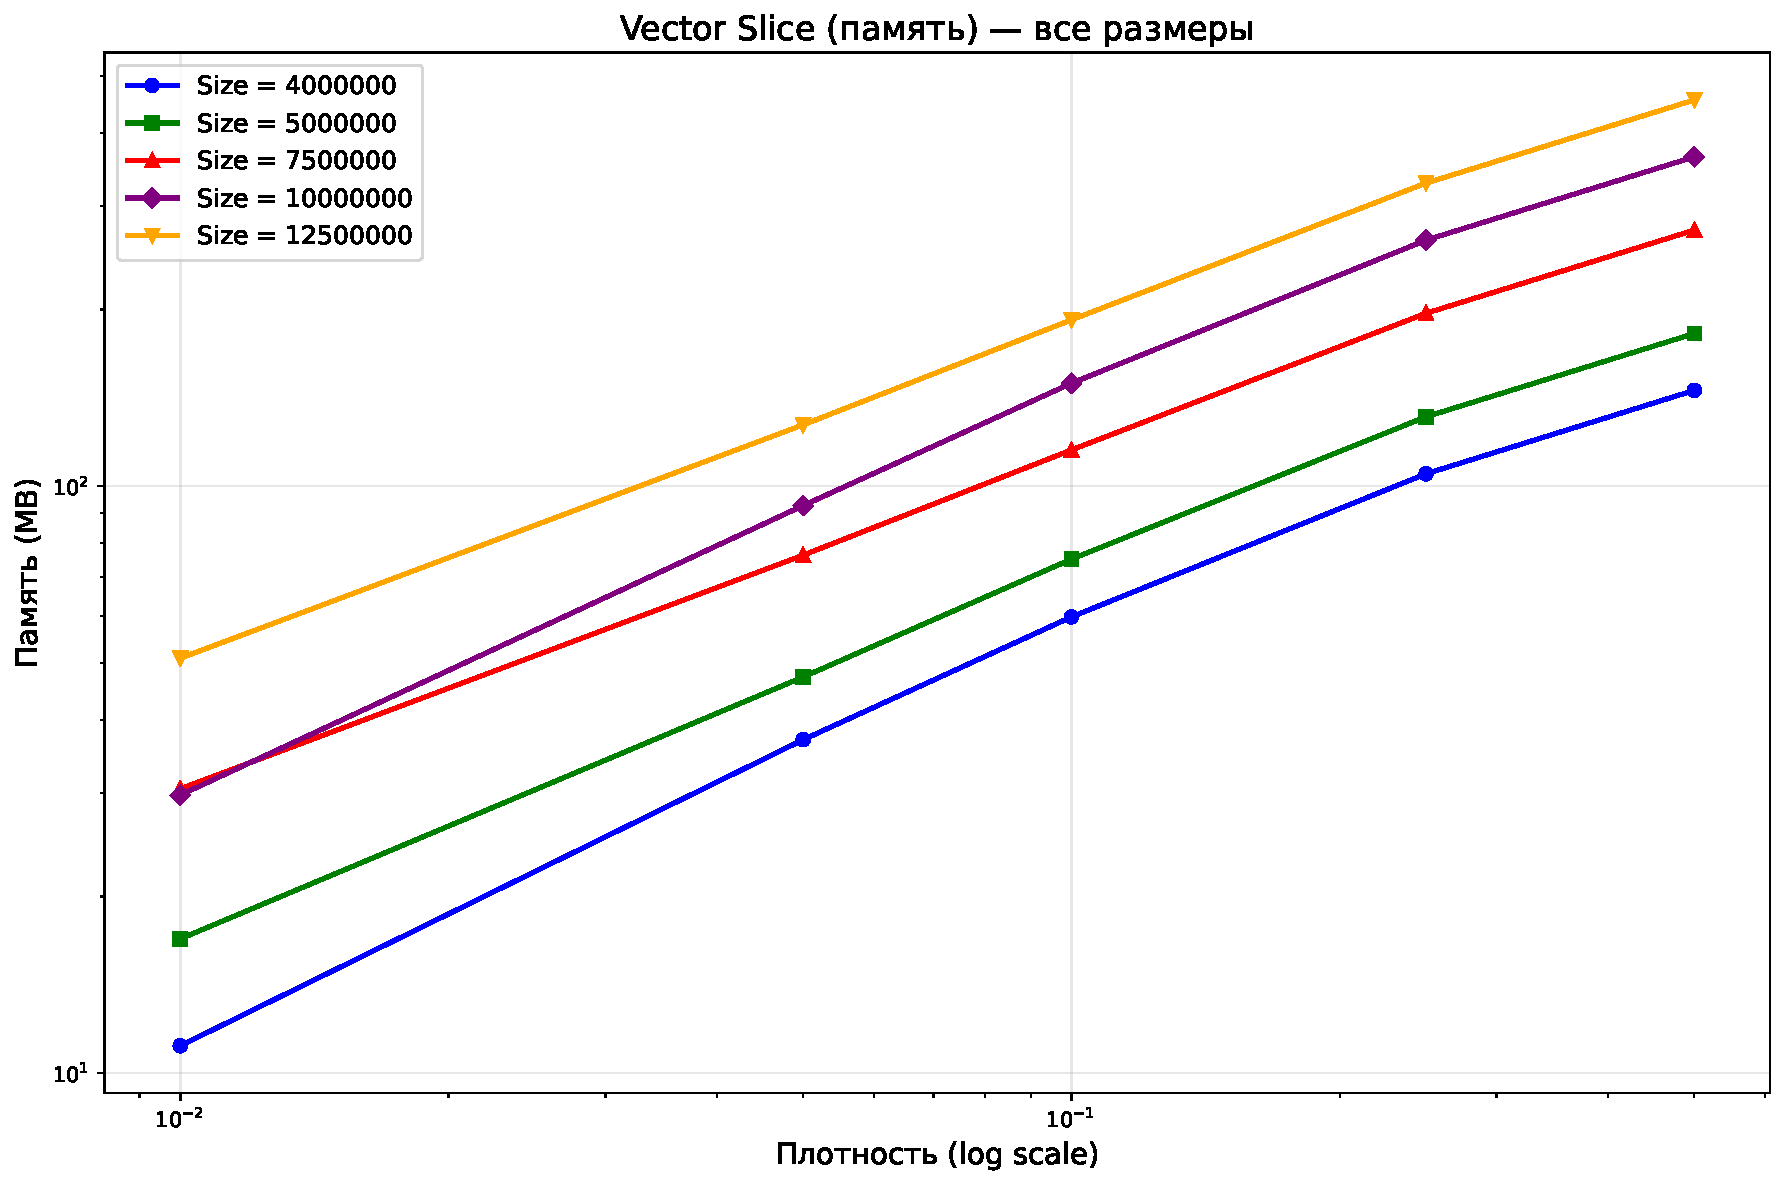
\includegraphics[width=0.9\textwidth]{vector_slice_memory_all_sizes.pdf}
    \caption{VectorSlice: объём выделенной памяти в зависимости от плотности для различных размеров}
    \label{fig:vector_slice_memory_all_sizes}
\end{figure}

Из рисунков видно, что при плотностях 0.25--0.5 увеличение размера приводит примерно к пропорциональному росту времени и объёма выделенной памяти.

\textbf{Matrix.slice.} Цель этого эксперимента~--- проверить, как время выполнения \texttt{Matrix.slice} зависит от размера матрицы и плотности. В эксперименте при каждом фиксированном значении плотности изменялся размер матрицы, а затем оценивалась степень зависимости времени от размера. Наблюдаемые экспериментальные степени при разных плотностях согласуются с квадратичным масштабированием по размеру матрицы. Отдельно изменение плотности исследовалось на графиках зависимости времени от плотности.

Для проверки теоретической оценки \(O(B \log N)\) была построена регрессия времени от предиктора \(\text{Size}^2 \cdot \log_2(\text{Size})\). Полученные значения \(k\) лежат в диапазоне 0.96--1.13 в зависимости от плотности, что согласуется с теоретическим значением \(k = 1\). Значения \(R^2\) превышают 0.85 во всех случаях и достигают 0.997 при плотности 0.5, что подтверждает адекватность модели. Таким образом, \texttt{Matrix.slice} согласуется с оценкой \(O(B \log N)\) во всём диапазоне исследованных плотностей.

\begin{figure}[H]
    \centering
    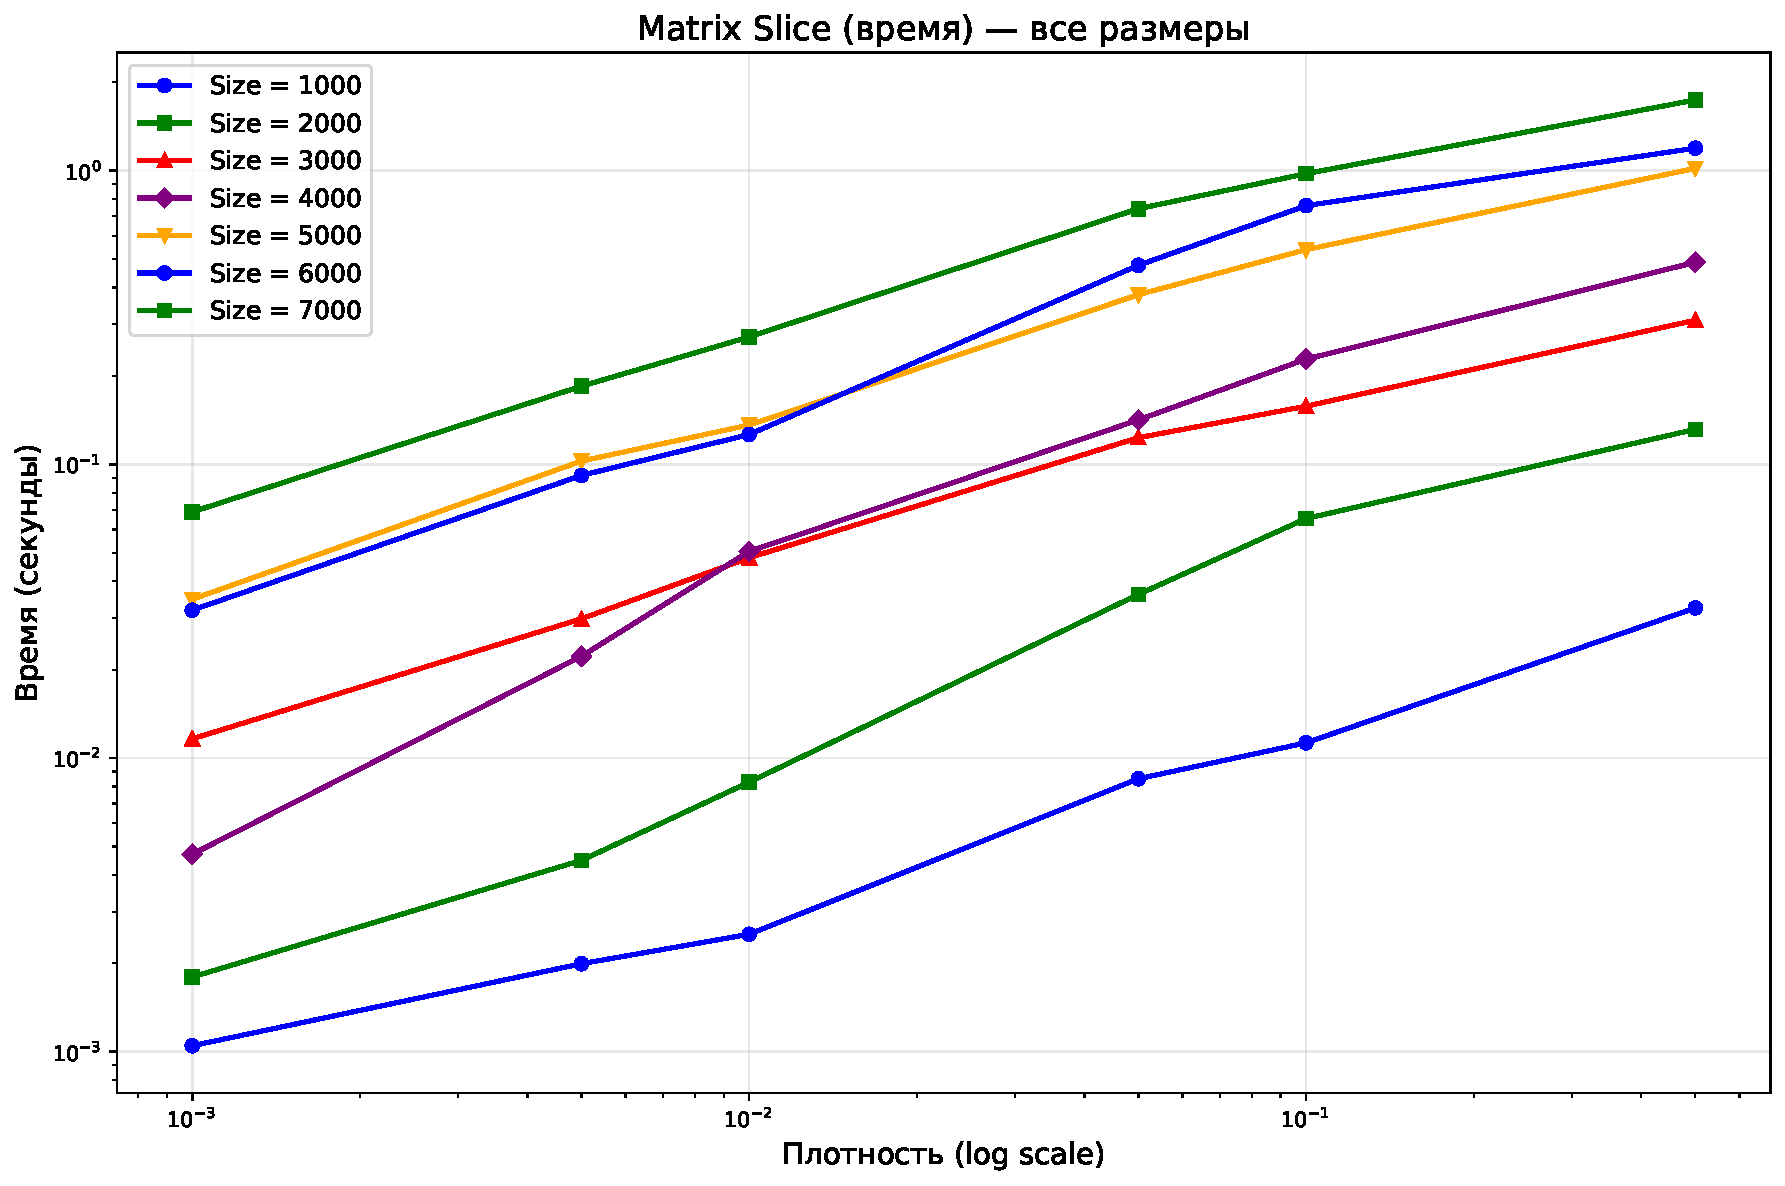
\includegraphics[width=0.9\textwidth]{matrix_slice_time_all_sizes.pdf}
    \caption{MatrixSlice: время выполнения в зависимости от плотности для различных размеров}
    \label{fig:matrix_slice_time_all_sizes}
\end{figure}

\begin{figure}[H]
    \centering
    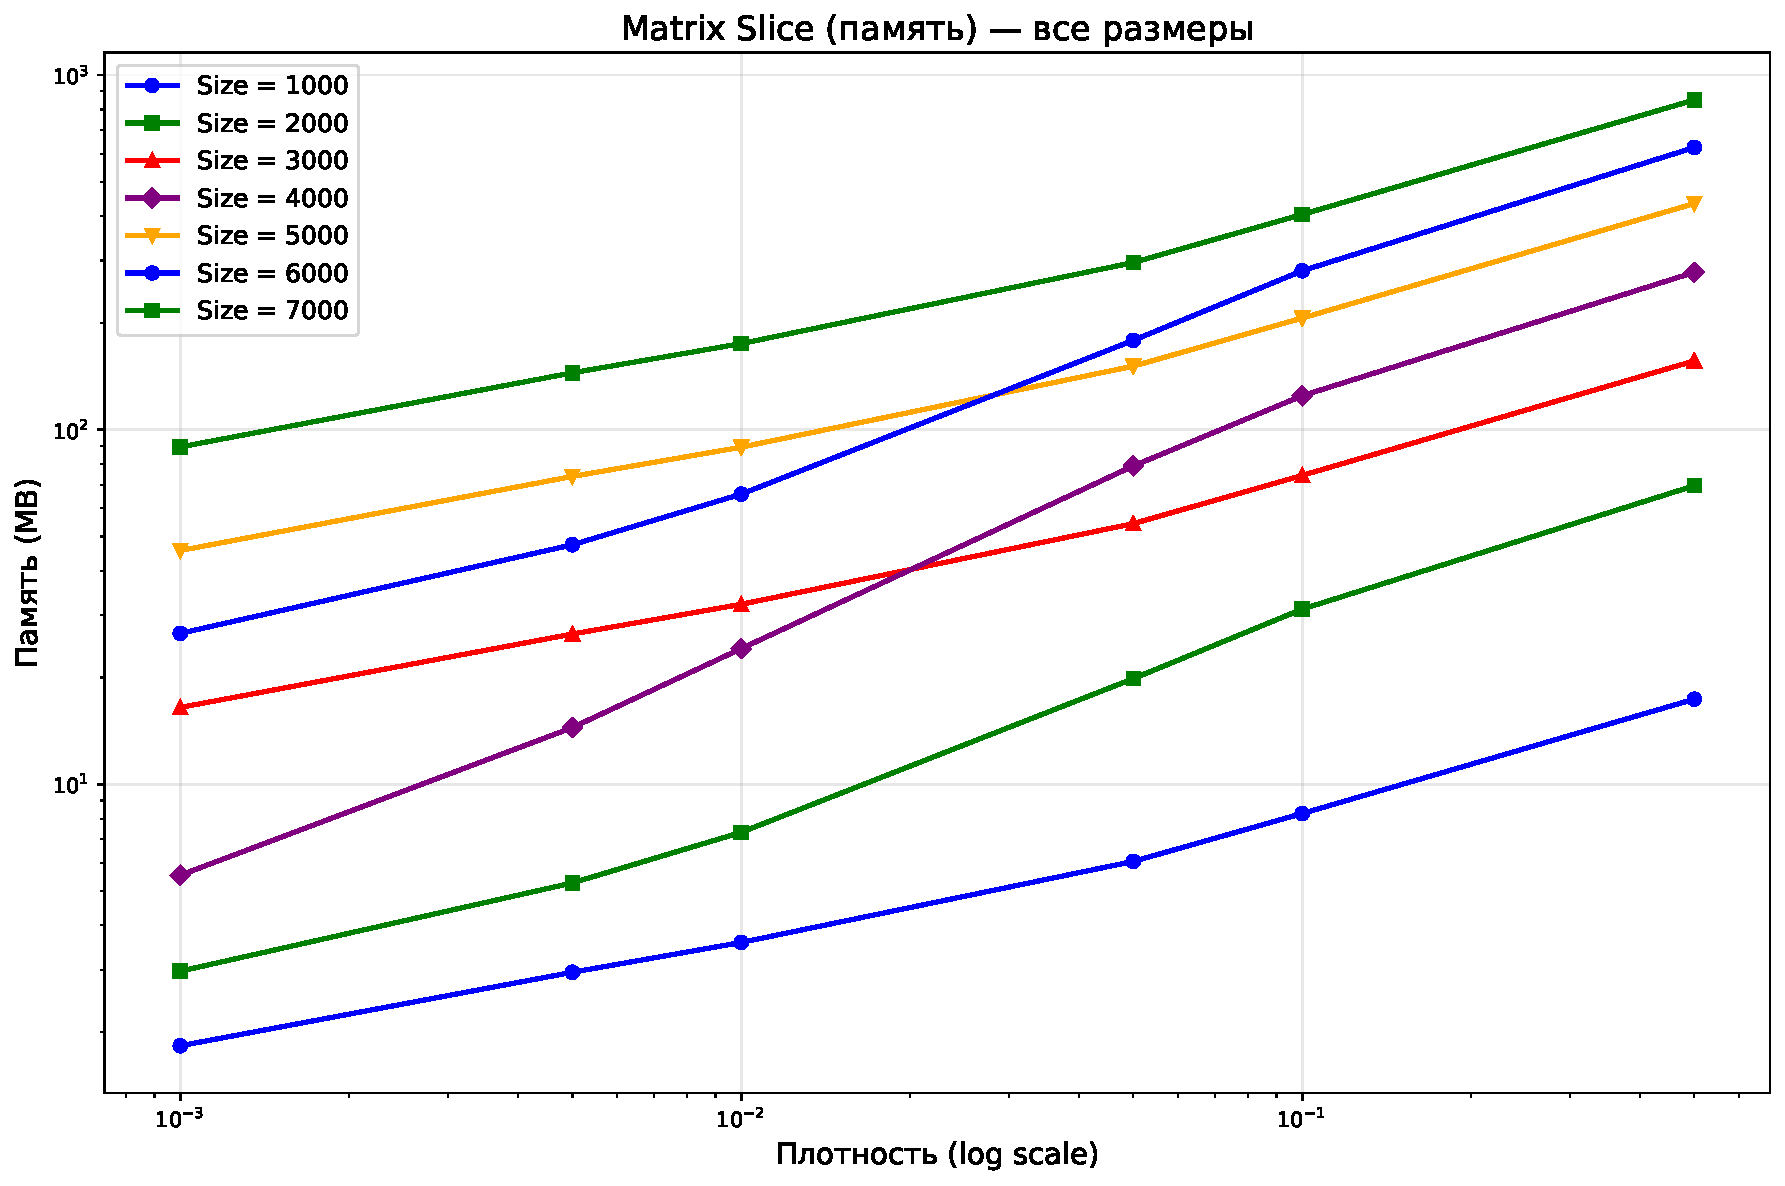
\includegraphics[width=0.9\textwidth]{matrix_slice_memory_all_sizes.pdf}
    \caption{MatrixSlice: объём выделенной памяти в зависимости от плотности для различных размеров}
    \label{fig:matrix_slice_memory_all_sizes}
\end{figure}

\textbf{Влияние выравнивания границ среза на производительность}
\label{sec:alignment}

Цель этого эксперимента~--- проверить влияние выравнивания границ среза относительно структуры квадрантного дерева на производительность.

В основном бенчмарке \texttt{Matrix.slice} были обнаружены немонотонности: при плотности 0.001 матрица 3000×3000 работала медленнее (в среднем 11.6 мс), чем 4000×4000 (4.7 мс), а при плотности 0.005 матрица 5000×5000 (101.8 мс)~--- медленнее, чем 6000×6000 (92.4 мс). Наблюдаемую немонотонность нельзя объяснить только изменением размера; отдельный эксперимент показывает существенное влияние выравнивания границ среза относительно структуры дерева.

Для проверки этой гипотезы был проведён отдельный диагностический эксперимент: фиксировался размер матрицы (4096×4096) и размер среза (2048), но менялось смещение начала среза (StartOffset = 0, 1, 512, 1024, 1536, 2048). Результаты показаны на рис.~\ref{fig:matrix_slice_align_time_vs_density}.

При плотности 0.001 смещение на 1 (StartOffset = 1) увеличивает время выполнения в 17 раз (с 2.5 мс до 43 мс) и объём выделенной памяти (Allocated) в 19 раз (с 3.8 МБ до 73.6 МБ). С ростом плотности относительный выигрыш от выравнивания уменьшается: при плотности 0.5 различие по времени остаётся заметным (примерно 1.78$\times$), тогда как различие по Allocated становится малым (около 1.04$\times$). Это объясняется тем, что при увеличении плотности возрастает доля работы, связанной с обработкой плотной части результата, поэтому вклад выравнивания снижается.

Для вектора аналогичный эксперимент показал значительно более слабый эффект (максимальное соотношение 4.7$\times$ при плотности 0.001). Это связано с одномерной структурой бинарного дерева: при плохой выровненности затрагиваются только одномерные координаты, тогда как в квадрантном дереве нарушение границ происходит одновременно по двум координатам.

Таким образом, наблюдаемая немонотонность объясняется чувствительностью алгоритма к выравниванию границ среза.

\begin{figure}[H]
    \centering
    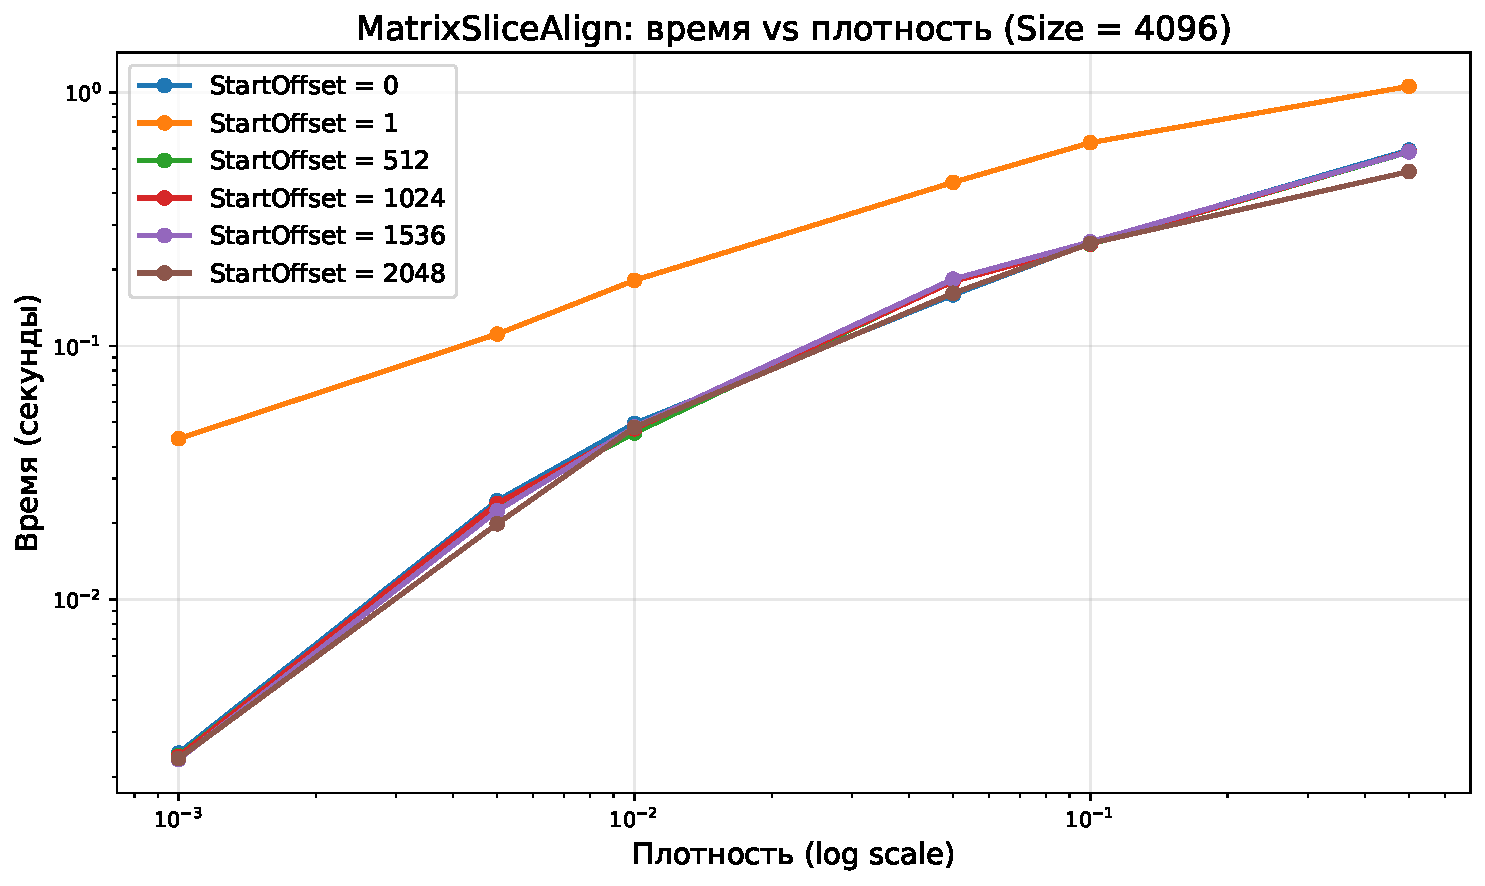
\includegraphics[width=0.9\textwidth]{matrix_slice_align_time_vs_density.pdf}
    \caption{MatrixSliceAlign: время выполнения для различных смещений (StartOffset)}
    \label{fig:matrix_slice_align_time_vs_density}
\end{figure}

\begin{figure}[H]
    \centering
    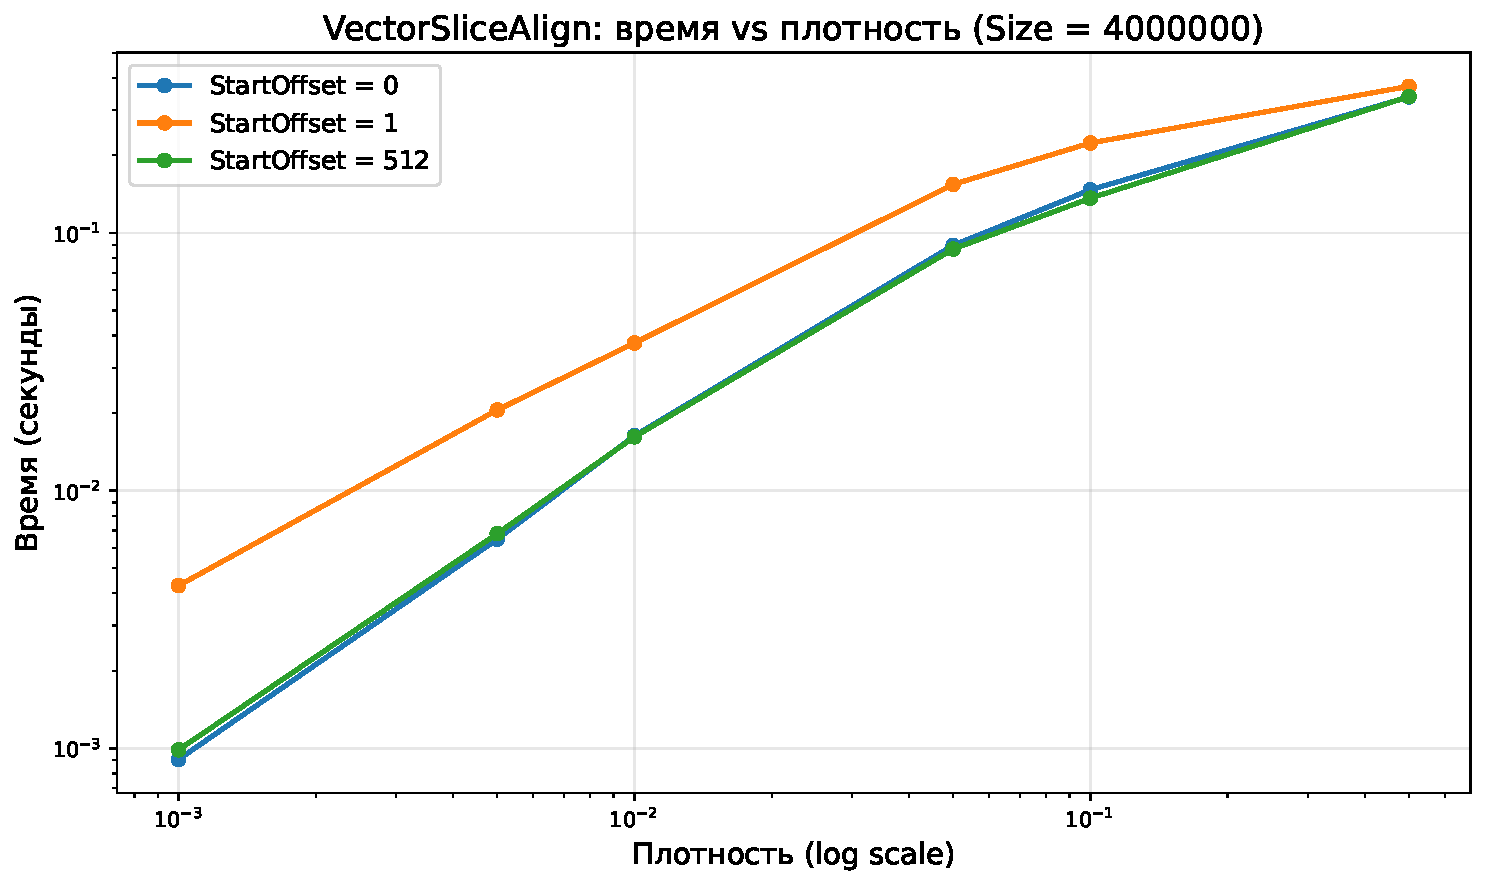
\includegraphics[width=0.9\textwidth]{vector_slice_align_time_vs_density.pdf}
    \caption{VectorSliceAlign: время выполнения для различных смещений (StartOffset)}
    \label{fig:vector_slice_align_time_vs_density}
\end{figure}

Из рисунков видно, что эффект выравнивания максимален при малой плотности и уменьшается с ростом плотности, что согласуется с гипотезой о влиянии структуры дерева.

\subsection{Выводы из экспериментов}

Проведённые эксперименты показали поведение, соответствующее теоретическим оценкам исследованных операций:
\begin{itemize}
    \item для \texttt{reduceCols} уточнённая теоретическая оценка \(O(U + nnz \cdot \log n)\) согласуется с экспериментальными данными (наклон \(k = 0.99\)--\(1.03\)).
    \item прямая редукция по столбцам оказалась быстрее подхода с транспонированием на всех 30 реальных матрицах, медианное ускорение составляет 1.74$\times$;
    \item для \texttt{kroneckerProduct} значение \(k = 0.89\) согласуется с выдвинутой теоретической оценкой \(O(nnz(A) \cdot nnz(B))\);
    \item для \texttt{Matrix.slice} и \texttt{Vector.slice} наклон регрессии \(k\) близок к единице при плотностях \(\ge 0.1\), что подтверждает оценку \(O(B \log N)\);
    \item выявлено влияние выравнивания границ среза на производительность \texttt{Vector.slice} и \texttt{Matrix.slice}; для квадрантного дерева эффект существенно сильнее.
\end{itemize}

\section*{Заключение}

В ходе выполнения работы в соответствии с техническим заданием проекта LamaGraph получены следующие результаты:

\begin{itemize}
    \item реализована операция взятия среза для вектора (\texttt{Vector.slice});
    \item реализована операция взятия среза для матрицы (\texttt{Matrix.slice});
    \item реализованы редукции матрицы по строкам (\texttt{reduceRows});
    \item реализованы редукции матрицы по столбцам (\texttt{reduceCols});
    \item реализовано произведение Кронекера для двух разреженных матриц (\texttt{kroneckerProduct});
    \item реализовано поэлементное отображение для матрицы (\texttt{Matrix.map});
    \item разработано 66 модульных тестов, покрывающих основные сценарии;
    \item экспериментально показано, что поведение исследованных операций согласуется с теоретическими оценками сложности;
    \item показано, что прямая редукция по столбцам быстрее подхода с транспонированием на всех 30 реальных матрицах (медианное ускорение 1.74$\times$).
\end{itemize}

Исходный код доступен в пулл-реквесте: \url{https://github.com/Lamagraph/QTreeFSharp/pull/18}. Разработанные операции могут быть использованы для реализации графовых алгоритмов в рамках дальнейшего развития проекта LamaGraph.

\begin{thebibliography}{99}
\bibitem{qtreefsharp} Исходный код проекта QTreeFSharp. URL: \url{https://github.com/Lamagraph/QTreeFSharp}

\bibitem{benchmarkdotnet} Официальная документация инструмента профилирования BenchmarkDotNet. URL: \url{https://benchmarkdotnet.org/}

\bibitem{fsharpdocs} Документация по языку F\#. URL: \url{https://learn.microsoft.com/ru-ru/dotnet/fsharp/}

\bibitem{suitesparse} Коллекция разреженных матриц SuiteSparse. URL: \url{https://sparse.tamu.edu/}
\end{thebibliography}

\end{document}
